%

% TODO: SDF vs SFD typo factory!

\documentclass[twocolumn]{amsart}
\usepackage[top=0.75in, left=0.65in, right=0.65in, bottom=0.6in]{geometry}

\usepackage{url}
% \usepackage{code}
% \usepackage{cite}
\usepackage{latexsym}
\usepackage{amsmath}
\usepackage{amssymb}
\usepackage{graphicx}
\usepackage{chessboard}
% IPA symbols. safe turns off overrides for like \! which I still want
\usepackage[safe]{tipa}

% \usepackage{chessfs}
\usepackage{adjustbox}

\usepackage[most]{tcolorbox}

\interfootnotelinepenalty=0

% lets me explicitly set a. or 1. etc. as enum label
\usepackage{enumitem}

\pagestyle{empty}

\usepackage{ulem}
% go back to italics for emphasis, though
\normalem

\usepackage{natbib}

\setlength{\footnotesep}{2em}

% \newcommand\comment[1]{}
\newcommand\sfrac[2]{\!{}\,^{#1}\!/{}\!_{#2}}

\begin{document}

\title{Lowestcase and Uppestcase letters: Further adventures in Derp Learning}
\author{Dr.~Tom~Murphy~VII~Ph.D.}\thanks{
Copyright \copyright\ 2021 the Regents of the Wikiplia Foundation.
Appears in SIGBOVIK~2021 with the
OS2TypoLinegap of the Association for Computational Heresy; {\em IEEEEEE!}
press, Verlag-Verlag volume no.~0x40-2A. 1 em}

\setchessboard{showmover=false}

\newcommand\makelowercase{{\sf make\_lowercase}}
\newcommand\makeuppercase{{\sf make\_uppercase}}

\renewcommand\th{\ensuremath{{}^{\textrm{th}}}}
\newcommand\st{\ensuremath{{}^{\textrm{st}}}}
\newcommand\rd{\ensuremath{{}^{\textrm{rd}}}}
\newcommand\nd{\ensuremath{{}^{\textrm{nd}}}}
\newcommand\at{\ensuremath{\scriptstyle @}}

\date{1 April 2021}

\maketitle \thispagestyle{empty}

\sloppypar


\section{Introduction}

Have you ever been writing something on the internet and wanted to convey
that you ARE FEELING ANGRY? Conversely, have you ever fired back a super
quick dm and u wanted to make it clear that it was like super ca\textipa{Z}
and so u didnt use ne capitals or punctuation dots except 4 that one place
where u needed to use the international phonetic alphabet because u dont
no how to write ca\textipa{Z} as in short for casual without it lol

If so, you made use of the fact that all letters have UPPERCASE
VERSIONS (e.g.~signifying ANGER) and lowercase versions
(e.g.~signifying u dont care lol). These dimensions have other uses,
for example, it is polite to start a person's name with a capital
letter to show that you took the time to regard their humanity (as it
takes extra work to press the caps lock key, press the first letter of
their name, and then press ther caps lock key again to turn it off).
In German, Nouns start with uppercase Letters, signifying Superiority
over other grammatical Categories like Verbs and Adjectives. Lowercase
letters can be used to conserve printer ink. Actually, I'm not sure that
lowercase letters have any other uses, but let's just roll with it.

The thing is: What if I'm even MORE ANGRY THAN I WAS BEFORE? There are
some standard sorts of typographic emphasis, like I can be {\bf BOLD
  ANGRY} or \textbf{\textit{\large BIG BOLD ITALIC UNDERLINE ANGRY}}
or { \Large \textbf{\textit{\uuline{COMBINE A LOT OF THESE ANGERS}}}},
each with its own nuances, depending on the cascading style sheet or
LaTeX class file. To be even more casual than lowercase, u can learn 2
write like this, and {\scriptsize shrink away} and also \sout{cross
  out ur words in shame in advance of them even being read}, but there
are few other options for de-emphasis. Plus, when I'm FEELING PRETTY
ANGRY, TOM, how do I capitalize that already-capitalized T in order to
show the proper reverence for your humanity?

This paper is about unshackling this dimension of human expression by
introducing letterforms further along the uppercase and lowercase
dimensions. Basically, we want to know what the upper{\it er}case
version of uppercase T is, and a lower{\it er}case version of
lowercase t is.

\subsection{Induction}

Today we're just concerned with English letters, of which there are
only 26. To create an upperercase and lowerercase alphabet by hand is
O(52 pick up), which for a guy who likes drawing letters anyway and
who alphabetized Star~Wars for fun, is not much to ask. In fact I
drew such alphabets in Figure~\ref{fig:manual} just now.

\begin{figure}[ht]
% \includegraphics[width=0.9 \linewidth]{manual}
\caption{TODO} \label{fig:manual}
\end{figure}

But, why do easy fun things by hand when you can build a complicated
automatic solution which produces much worse results? Well, there is
no good reason. I could claim that this allows us to automatically
upperercase any font, which is true, but the results are at best
moderately letter-like lumps. In principle there are several other
interesting things we can do, like apply the function over and over to
approach the uppestcase and lowestcase letters. This sounds fun, but
the results themselves are not going to impress. But the story of
getting there may be interesting, and even as it turns out to be
``derp learning,'' there will be opportunities for more good puns. So
let's just roll with it!


\section{Capital A Artificial Intelligence}

% XXX want some macro for referring to a letter's shape, maybe
% with a box around it?

\newcommand\letterform[1]{\tcbox[
    nobeforeafter,
    tcbox raise base,
    top=0pt,bottom=0pt,left=-1pt,right=-1pt,
    left skip=1pt,
    right skip=1pt,
    arc=2pt,outer arc=2pt,
    boxrule=0.15mm,
    colback=white,
    colframe=white!50!black
    ]{\textrm{#1}}}

%     leftrule=0.2pt,rightrule=0.2pt,toprule=0.2pt,bottomrule=0.2pt,
%     enhanced jigsaw,
%    borderline horizontal={0.2pt}{0pt}{dashed},
%    borderline vertical={0.2pt}{0pt}{dashed}


We want to machine-learn two functions, \makelowercase\ and
\makeuppercase. Each takes a letterform and returns a letterform (we
can choose how these are represented) and does the needful, e.g.
\makelowercase(\letterform{A}) should return \letterform{a}. In order to learn this function, we'll at least need a lot of
examples to use as training data. A training example for
\makelowercase\ is a letterform and its expected corresponding
lowercase one. We can ``easily'' find a large amount of examples by
using existing fonts, and pairing their \letterform{A} with their
\letterform{a}, and so on for all 26 letters, and symmetrically for
\makeuppercase.

However, if we only give uppercase letters to \makelowercase, it
may very well learn how to generate the corresponding lowercase letter
but be unable to do anything interesting for other letterforms. This
is a problem because we want to use this function to see
what e.g.~\makelowercase(\letterform{a}) is.

This is not (only) the problem of overfitting. An overfit model could
work well on the letter \letterform{A} from one font (because it has
seen that font before) but fail on \letterform{A} from a new font. The
property that we want is that the learned function can also produce an
interesting result on a shape it's never seen before, like
\letterform{\textipa{Z}}\,. That is, it has generalized the idea of
``how to make a shape lowercase,'' not simply ``how to make a capital
A shape lowercase.''

The problem with this is that we don't have any training data other
than existing fonts to tell us what the lowercase of some arbitrary
shape should look like. Without examples of this form, the problem is
unconstrained. \makelowercase\ could learn to generate empty output
for anything it doesn't recognize as a capital letter, and still have
perfect performance on the training and test set. It is hard to
generate training data of this form (even by hand) as we don't have
much idea {\em a priori} of what a lowerercase \letterform{a} should
look like (except for e.g.~One Artist's Impression from
Figure~\ref{fig:manual}).

\newcommand\trainingexample[2]{$\langle$\letterform{#1}$,\,$\letterform{#2}$\rangle$}

\newcommand\weirdcharlo{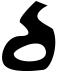
\includegraphics[width=0.8em]{weirdchar-lo}}
\newcommand\weirdcharup{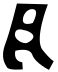
\includegraphics[width=0.8em]{weirdchar-up}}

This brings us to the one decent idea in this paper (which by the way
only sort of works, but let's just roll with it). We can at least
express one characteristic property of the \makelowercase\ function
that ought to be true even for letterforms we don't have examples of:
It ought to be the inverse of \makeuppercase. So, we train these two
models in tandem. \makelowercase\ is fed training examples from the
sample fonts like \trainingexample{Q}{q} etc.~and \makeuppercase\ gets
\trainingexample{e}{E} etc.~as expected. We also run the current
version of \makeuppercase\ on some letter-like shapes, which produces
some other shape. For example, say that
\makeuppercase(\letterform{\weirdcharlo}) outputs
\letterform{\weirdcharup}. We have no idea if this is good or not, so
we don't update the model. However, we {\em do} provide the training
example to \trainingexample{\weirdcharup}{\weirdcharlo} to the
\makelowercase\ training queue and penalize {\em it} if it did not
predict \letterform{\weirdcharup}. In this way, whatever \makeuppercase\ is
doing, we ask \makelowercase\ to learn the inverse. We of course also
simultaneously do the symmetric thing, using the output of
\makelowercase\ to create training examples for
\makeuppercase\ (Figure~\ref{fig:cotraining}).

\begin{figure}[ht]
% \includegraphics[width=0.9 \linewidth]{manual}
\caption{TODO cotraining} \label{fig:cotraining}
\end{figure}

Because \makelowercase\ is getting training examples of
uppercase/lowercase pairs from real fonts, it remains grounded on real
letters. It is also free to generate new shapes in the open domain
(outside \letterform{A}--\letterform{Z}). However, it is penalized if
its behavior is not the inverse of whatever \makeuppercase\ is
currently doing. And since we do the symmetric thing for
\makeuppercase\, there is a (slow) feedback loop between the two
models that keeps them from straying too far from the grounded
examples. The idea is that this allows them to do some creative
generalization outside their native domains, but in a way that
still has some constraint.

In practice, we don't feed arbitrary shapes to the models. We
just need something letter-like, and in fact we have a large
collection of letter-like shapes among our existing fonts. So
we pass already-lowercase shapes to \makelowercase, in order
to generate inversion examples for training \makeuppercase.
These shapes are clearly letter-like (they {\em are} letters) and
are also of interest to us anyway, since we want to try to
generate lowerercase and upperercase letters with these models.


% $\langle\,$\letterform{Q}, \letterform{q}$\,\rangle$
% $\langle\,$\letterform{e}, \letterform{E}$\,\rangle$

\section{1000001 Free Fonts}

% no copyright intended

% (lowercase i intelligence: redi)

% The care and feeding of sparse matrices

% Perfect letters, hallucinated

% autotracing

% CAPS LOCK, LOCK, CAPTAIN'S LOCK

% when two letters coincide, a shift-reduce conflict

% cool s

% lowercase uppercase letters etc.

\nocite{murphy2019blind}
\nocite{murphy2019eloworld}

\bibliography{lowercase}{}
\bibliographystyle{plain}

\end{document}

